\documentclass[]{book}
\usepackage{lmodern}
\usepackage{amssymb,amsmath}
\usepackage{ifxetex,ifluatex}
\usepackage{fixltx2e} % provides \textsubscript
\ifnum 0\ifxetex 1\fi\ifluatex 1\fi=0 % if pdftex
  \usepackage[T1]{fontenc}
  \usepackage[utf8]{inputenc}
\else % if luatex or xelatex
  \ifxetex
    \usepackage{mathspec}
  \else
    \usepackage{fontspec}
  \fi
  \defaultfontfeatures{Ligatures=TeX,Scale=MatchLowercase}
\fi
% use upquote if available, for straight quotes in verbatim environments
\IfFileExists{upquote.sty}{\usepackage{upquote}}{}
% use microtype if available
\IfFileExists{microtype.sty}{%
\usepackage{microtype}
\UseMicrotypeSet[protrusion]{basicmath} % disable protrusion for tt fonts
}{}
\usepackage[margin=1in]{geometry}
\usepackage{hyperref}
\hypersetup{unicode=true,
            pdftitle={Collaborative Data Science Practices},
            pdfauthor={Will Beasley},
            pdfborder={0 0 0},
            breaklinks=true}
\urlstyle{same}  % don't use monospace font for urls
\usepackage{natbib}
\bibliographystyle{apalike}
\usepackage{color}
\usepackage{fancyvrb}
\newcommand{\VerbBar}{|}
\newcommand{\VERB}{\Verb[commandchars=\\\{\}]}
\DefineVerbatimEnvironment{Highlighting}{Verbatim}{commandchars=\\\{\}}
% Add ',fontsize=\small' for more characters per line
\usepackage{framed}
\definecolor{shadecolor}{RGB}{248,248,248}
\newenvironment{Shaded}{\begin{snugshade}}{\end{snugshade}}
\newcommand{\AlertTok}[1]{\textcolor[rgb]{0.94,0.16,0.16}{#1}}
\newcommand{\AnnotationTok}[1]{\textcolor[rgb]{0.56,0.35,0.01}{\textbf{\textit{#1}}}}
\newcommand{\AttributeTok}[1]{\textcolor[rgb]{0.77,0.63,0.00}{#1}}
\newcommand{\BaseNTok}[1]{\textcolor[rgb]{0.00,0.00,0.81}{#1}}
\newcommand{\BuiltInTok}[1]{#1}
\newcommand{\CharTok}[1]{\textcolor[rgb]{0.31,0.60,0.02}{#1}}
\newcommand{\CommentTok}[1]{\textcolor[rgb]{0.56,0.35,0.01}{\textit{#1}}}
\newcommand{\CommentVarTok}[1]{\textcolor[rgb]{0.56,0.35,0.01}{\textbf{\textit{#1}}}}
\newcommand{\ConstantTok}[1]{\textcolor[rgb]{0.00,0.00,0.00}{#1}}
\newcommand{\ControlFlowTok}[1]{\textcolor[rgb]{0.13,0.29,0.53}{\textbf{#1}}}
\newcommand{\DataTypeTok}[1]{\textcolor[rgb]{0.13,0.29,0.53}{#1}}
\newcommand{\DecValTok}[1]{\textcolor[rgb]{0.00,0.00,0.81}{#1}}
\newcommand{\DocumentationTok}[1]{\textcolor[rgb]{0.56,0.35,0.01}{\textbf{\textit{#1}}}}
\newcommand{\ErrorTok}[1]{\textcolor[rgb]{0.64,0.00,0.00}{\textbf{#1}}}
\newcommand{\ExtensionTok}[1]{#1}
\newcommand{\FloatTok}[1]{\textcolor[rgb]{0.00,0.00,0.81}{#1}}
\newcommand{\FunctionTok}[1]{\textcolor[rgb]{0.00,0.00,0.00}{#1}}
\newcommand{\ImportTok}[1]{#1}
\newcommand{\InformationTok}[1]{\textcolor[rgb]{0.56,0.35,0.01}{\textbf{\textit{#1}}}}
\newcommand{\KeywordTok}[1]{\textcolor[rgb]{0.13,0.29,0.53}{\textbf{#1}}}
\newcommand{\NormalTok}[1]{#1}
\newcommand{\OperatorTok}[1]{\textcolor[rgb]{0.81,0.36,0.00}{\textbf{#1}}}
\newcommand{\OtherTok}[1]{\textcolor[rgb]{0.56,0.35,0.01}{#1}}
\newcommand{\PreprocessorTok}[1]{\textcolor[rgb]{0.56,0.35,0.01}{\textit{#1}}}
\newcommand{\RegionMarkerTok}[1]{#1}
\newcommand{\SpecialCharTok}[1]{\textcolor[rgb]{0.00,0.00,0.00}{#1}}
\newcommand{\SpecialStringTok}[1]{\textcolor[rgb]{0.31,0.60,0.02}{#1}}
\newcommand{\StringTok}[1]{\textcolor[rgb]{0.31,0.60,0.02}{#1}}
\newcommand{\VariableTok}[1]{\textcolor[rgb]{0.00,0.00,0.00}{#1}}
\newcommand{\VerbatimStringTok}[1]{\textcolor[rgb]{0.31,0.60,0.02}{#1}}
\newcommand{\WarningTok}[1]{\textcolor[rgb]{0.56,0.35,0.01}{\textbf{\textit{#1}}}}
\usepackage{longtable,booktabs}
\usepackage{graphicx,grffile}
\makeatletter
\def\maxwidth{\ifdim\Gin@nat@width>\linewidth\linewidth\else\Gin@nat@width\fi}
\def\maxheight{\ifdim\Gin@nat@height>\textheight\textheight\else\Gin@nat@height\fi}
\makeatother
% Scale images if necessary, so that they will not overflow the page
% margins by default, and it is still possible to overwrite the defaults
% using explicit options in \includegraphics[width, height, ...]{}
\setkeys{Gin}{width=\maxwidth,height=\maxheight,keepaspectratio}
\IfFileExists{parskip.sty}{%
\usepackage{parskip}
}{% else
\setlength{\parindent}{0pt}
\setlength{\parskip}{6pt plus 2pt minus 1pt}
}
\setlength{\emergencystretch}{3em}  % prevent overfull lines
\providecommand{\tightlist}{%
  \setlength{\itemsep}{0pt}\setlength{\parskip}{0pt}}
\setcounter{secnumdepth}{5}
% Redefines (sub)paragraphs to behave more like sections
\ifx\paragraph\undefined\else
\let\oldparagraph\paragraph
\renewcommand{\paragraph}[1]{\oldparagraph{#1}\mbox{}}
\fi
\ifx\subparagraph\undefined\else
\let\oldsubparagraph\subparagraph
\renewcommand{\subparagraph}[1]{\oldsubparagraph{#1}\mbox{}}
\fi

%%% Use protect on footnotes to avoid problems with footnotes in titles
\let\rmarkdownfootnote\footnote%
\def\footnote{\protect\rmarkdownfootnote}

%%% Change title format to be more compact
\usepackage{titling}

% Create subtitle command for use in maketitle
\newcommand{\subtitle}[1]{
  \posttitle{
    \begin{center}\large#1\end{center}
    }
}

\setlength{\droptitle}{-2em}

  \title{Collaborative Data Science Practices}
    \pretitle{\vspace{\droptitle}\centering\huge}
  \posttitle{\par}
    \author{Will Beasley}
    \preauthor{\centering\large\emph}
  \postauthor{\par}
      \predate{\centering\large\emph}
  \postdate{\par}
    \date{2018-10-17}

\usepackage{booktabs}

\usepackage{amsthm}
\newtheorem{theorem}{Theorem}[chapter]
\newtheorem{lemma}{Lemma}[chapter]
\theoremstyle{definition}
\newtheorem{definition}{Definition}[chapter]
\newtheorem{corollary}{Corollary}[chapter]
\newtheorem{proposition}{Proposition}[chapter]
\theoremstyle{definition}
\newtheorem{example}{Example}[chapter]
\theoremstyle{definition}
\newtheorem{exercise}{Exercise}[chapter]
\theoremstyle{remark}
\newtheorem*{remark}{Remark}
\newtheorem*{solution}{Solution}
\begin{document}
\maketitle

{
\setcounter{tocdepth}{1}
\tableofcontents
}
\hypertarget{prerequisites}{%
\chapter{Prerequisites}\label{prerequisites}}

This is a \emph{sample} book written in \textbf{Markdown}. You can use
anything that Pandoc's Markdown supports, e.g., a math equation
\(a^2 + b^2 = c^2\).

The \textbf{bookdown} package can be installed from CRAN or Github:

\begin{Shaded}
\begin{Highlighting}[]
\KeywordTok{install.packages}\NormalTok{(}\StringTok{"bookdown"}\NormalTok{)}
\CommentTok{# or the development version}
\CommentTok{# devtools::install_github("rstudio/bookdown")}
\end{Highlighting}
\end{Shaded}

Remember each Rmd file contains one and only one chapter, and a chapter
is defined by the first-level heading \texttt{\#}.

To compile this example to PDF, you need XeLaTeX. You are recommended to
install TinyTeX (which includes XeLaTeX):
\url{https://yihui.name/tinytex/}.

\hypertarget{architecture}{%
\chapter{Architecture Principles}\label{architecture}}

\hypertarget{encapsulation}{%
\section{Encapsulation}\label{encapsulation}}

\hypertarget{leverage-team-members-strenghts-avoid-weaknesses}{%
\section{Leverage team member's strenghts \& avoid
weaknesses}\label{leverage-team-members-strenghts-avoid-weaknesses}}

\begin{enumerate}
\def\labelenumi{\arabic{enumi}.}
\tightlist
\item
  Focused code files
\item
  Metadata for content experts
\end{enumerate}

\hypertarget{scales}{%
\section{Scales}\label{scales}}

\begin{enumerate}
\def\labelenumi{\arabic{enumi}.}
\tightlist
\item
  Single source \& single analysis
\item
  Multiple sources \& multiple analyses
\end{enumerate}

\hypertarget{consistency}{%
\section{Consistency}\label{consistency}}

\begin{enumerate}
\def\labelenumi{\arabic{enumi}.}
\tightlist
\item
  Across Files
\item
  Across Languages
\item
  Across Projects
\end{enumerate}

\hypertarget{file-prototype}{%
\chapter{Prototypical File}\label{file-prototype}}

\hypertarget{clear-memory}{%
\section{Clear Memory}\label{clear-memory}}

\hypertarget{load-sources}{%
\section{Load Sources}\label{load-sources}}

\hypertarget{load-packages}{%
\section{Load Packages}\label{load-packages}}

\hypertarget{declare-globals}{%
\section{Declare Globals}\label{declare-globals}}

\hypertarget{load-data}{%
\section{Load Data}\label{load-data}}

\hypertarget{tweak-data}{%
\section{Tweak Data}\label{tweak-data}}

\hypertarget{unique-content}{%
\section{(Unique Content)}\label{unique-content}}

\hypertarget{verify-values}{%
\section{Verify Values}\label{verify-values}}

\hypertarget{specify-output-columns}{%
\section{Specify Output Columns}\label{specify-output-columns}}

\hypertarget{save-to-disk-or-database}{%
\section{Save to Disk or Database}\label{save-to-disk-or-database}}

\hypertarget{repo-prototype}{%
\chapter{Prototypical Repository}\label{repo-prototype}}

\url{https://github.com/wibeasley/RAnalysisSkeleton}

\hypertarget{analysis}{%
\section{Analysis}\label{analysis}}

\hypertarget{data-public}{%
\section{Data Public}\label{data-public}}

\begin{enumerate}
\def\labelenumi{\arabic{enumi}.}
\tightlist
\item
  Raw
\item
  Derived
\item
  Metadata
\item
  Database
\item
  Original
\end{enumerate}

\hypertarget{data-unshared}{%
\section{Data Unshared}\label{data-unshared}}

\hypertarget{documentation}{%
\section{Documentation}\label{documentation}}

\hypertarget{manipulation}{%
\section{Manipulation}\label{manipulation}}

\hypertarget{stitched-output}{%
\section{Stitched Output}\label{stitched-output}}

\hypertarget{utility}{%
\section{Utility}\label{utility}}

\hypertarget{data-at-rest}{%
\chapter{Data at Rest}\label{data-at-rest}}

\hypertarget{data-states}{%
\section{Data States}\label{data-states}}

\begin{enumerate}
\def\labelenumi{\arabic{enumi}.}
\tightlist
\item
  Raw
\item
  Derived

  \begin{enumerate}
  \def\labelenumii{\arabic{enumii}.}
  \tightlist
  \item
    Project-wide File on Repo
  \item
    Project-wide File on Protected File Server
  \item
    User-specific File on Protected File Server
  \item
    Project-wide Database
  \end{enumerate}
\item
  Original
\end{enumerate}

\hypertarget{data-containers}{%
\section{Data Containers}\label{data-containers}}

\begin{enumerate}
\def\labelenumi{\arabic{enumi}.}
\tightlist
\item
  csv
\item
  rds
\item
  SQLite
\item
  Central Enterprise database
\item
  Central REDCap database
\item
  Containers to avoid for raw/input

  \begin{enumerate}
  \def\labelenumii{\arabic{enumii}.}
  \tightlist
  \item
    Proprietary like xlsx, sas7bdat
  \end{enumerate}
\end{enumerate}

\hypertarget{patterns}{%
\chapter{Patterns}\label{patterns}}

\hypertarget{ellis}{%
\section{Ellis}\label{ellis}}

\hypertarget{arch}{%
\section{Arch}\label{arch}}

\hypertarget{ferry}{%
\section{Ferry}\label{ferry}}

\hypertarget{scribe}{%
\section{Scribe}\label{scribe}}

\hypertarget{analysis-1}{%
\section{Analysis}\label{analysis-1}}

\hypertarget{presentation--static}{%
\section{Presentation -Static}\label{presentation--static}}

\hypertarget{presentation--interactive}{%
\section{Presentation -Interactive}\label{presentation--interactive}}

\hypertarget{metadata}{%
\section{Metadata}\label{metadata}}

\hypertarget{security}{%
\chapter{Security \& Private Data}\label{security}}

\hypertarget{file-level-permissions}{%
\section{File-level permissions}\label{file-level-permissions}}

\hypertarget{database-permissions}{%
\section{Database permissions}\label{database-permissions}}

\hypertarget{public-private-repositories}{%
\section{Public \& Private
Repositories}\label{public-private-repositories}}

\begin{enumerate}
\def\labelenumi{\arabic{enumi}.}
\tightlist
\item
  Scrubbing GitHub history
\end{enumerate}

\hypertarget{automation}{%
\chapter{Automation}\label{automation}}

\hypertarget{flow-file-in-r}{%
\section{Flow File in R}\label{flow-file-in-r}}

\hypertarget{makefile}{%
\section{Makefile}\label{makefile}}

\hypertarget{ssis}{%
\section{SSIS}\label{ssis}}

\hypertarget{cron-jobs-task-scheduler}{%
\section{cron Jobs \& Task Scheduler}\label{cron-jobs-task-scheduler}}

\hypertarget{sink-log-files}{%
\section{Sink Log Files}\label{sink-log-files}}

\hypertarget{scaling-up}{%
\chapter{Scaling Up}\label{scaling-up}}

\hypertarget{data-storage}{%
\section{Data Storage}\label{data-storage}}

\begin{enumerate}
\def\labelenumi{\arabic{enumi}.}
\tightlist
\item
  Local File vs Conventional Database vs Redshift
\item
  Usage Cases
\end{enumerate}

\hypertarget{data-processing}{%
\section{Data Processing}\label{data-processing}}

\begin{enumerate}
\def\labelenumi{\arabic{enumi}.}
\tightlist
\item
  R vs SQL
\item
  R vs Spark
\end{enumerate}

\hypertarget{collaboration}{%
\chapter{Parallel Collaboration}\label{collaboration}}

\hypertarget{social-contract}{%
\section{Social Contract}\label{social-contract}}

\begin{enumerate}
\def\labelenumi{\arabic{enumi}.}
\tightlist
\item
  Issues
\item
  Organized Commits \& Coherent Diffs
\item
  Branch \& Merge Strategy
\end{enumerate}

\hypertarget{code-reviews}{%
\section{Code Reviews}\label{code-reviews}}

\begin{enumerate}
\def\labelenumi{\arabic{enumi}.}
\tightlist
\item
  Daily Reviews of PRs
\item
  Periodic Reviews of Files
\end{enumerate}

\hypertarget{remote}{%
\section{Remote}\label{remote}}

\begin{enumerate}
\def\labelenumi{\arabic{enumi}.}
\tightlist
\item
  Headset \& sharing screens
\end{enumerate}

\hypertarget{documentation}{%
\chapter{Documentation}\label{documentation}}

\hypertarget{team-wide}{%
\section{Team-wide}\label{team-wide}}

\hypertarget{project-specific}{%
\section{Project-specific}\label{project-specific}}

\hypertarget{dataset-origin-structure}{%
\section{Dataset Origin \& Structure}\label{dataset-origin-structure}}

\hypertarget{issues-tasks}{%
\section{Issues \& Tasks}\label{issues-tasks}}

\hypertarget{flow-diagrams}{%
\section{Flow Diagrams}\label{flow-diagrams}}

\hypertarget{setting-up-new-machine}{%
\section{Setting up new machine}\label{setting-up-new-machine}}

(\href{https://github.com/OuhscBbmc/RedcapExamplesAndPatterns/blob/master/DocumentationGlobal/ResourcesInstallation.md}{example})

\hypertarget{publication}{%
\chapter{Publishing Results}\label{publication}}

\hypertarget{to-other-analysts}{%
\section{To Other Analysts}\label{to-other-analysts}}

\hypertarget{to-researchers-content-experts}{%
\section{To Researchers \& Content
Experts}\label{to-researchers-content-experts}}

\hypertarget{to-technical-phobic-audiences}{%
\section{To Technical-Phobic
Audiences}\label{to-technical-phobic-audiences}}

\hypertarget{testing-and-validation}{%
\chapter{Testing, Validation, \& Defensive
Programming}\label{testing-and-validation}}

\hypertarget{testing-functions}{%
\section{Testing Functions}\label{testing-functions}}

\hypertarget{defensive-programming}{%
\section{Defensive Programming}\label{defensive-programming}}

\begin{enumerate}
\def\labelenumi{\arabic{enumi}.}
\tightlist
\item
  Throwing errors
\end{enumerate}

\hypertarget{validator}{%
\section{Validator}\label{validator}}

\begin{enumerate}
\def\labelenumi{\arabic{enumi}.}
\tightlist
\item
  Benefits for Analysts
\item
  Benefits for Data Collectors
\end{enumerate}

\hypertarget{troubleshooting}{%
\chapter{Troubleshooting and Debugging}\label{troubleshooting}}

\hypertarget{finding-help}{%
\section{Finding Help}\label{finding-help}}

\begin{enumerate}
\def\labelenumi{\arabic{enumi}.}
\tightlist
\item
  Within your group (eg, Thomas and REDCap questions)
\item
  Within your university (eg, SCUG)
\item
  Outside (eg, Stack Overflow; GitHub issues)
\end{enumerate}

\hypertarget{debugging}{%
\section{Debugging}\label{debugging}}

\begin{enumerate}
\def\labelenumi{\arabic{enumi}.}
\tightlist
\item
  \texttt{traceback()}, \texttt{browser()}, etc
\end{enumerate}

\hypertarget{establishing-workstation}{%
\chapter{Considerations when Selecting
Tools}\label{establishing-workstation}}

\url{https://github.com/OuhscBbmc/RedcapExamplesAndPatterns/blob/master/DocumentationGlobal/ResourcesInstallation.md}

\hypertarget{required-installation}{%
\section{Required Installation}\label{required-installation}}

\hypertarget{recommended-installation}{%
\section{Recommended Installation}\label{recommended-installation}}

\hypertarget{optional-installation}{%
\section{Optional Installation}\label{optional-installation}}

\hypertarget{asset-locations}{%
\section{Asset Locations}\label{asset-locations}}

\hypertarget{tools}{%
\chapter{Considerations when Selecting Tools}\label{tools}}

\hypertarget{general}{%
\section{General}\label{general}}

\begin{enumerate}
\def\labelenumi{\arabic{enumi}.}
\tightlist
\item
  The Component's Goal
\item
  Current Skillset of Team
\item
  Desired Future Skillset of Team
\item
  Skillset of Audience
\end{enumerate}

\hypertarget{languages}{%
\section{Languages}\label{languages}}

\hypertarget{r-packages}{%
\section{R Packages}\label{r-packages}}

\hypertarget{database}{%
\section{Database}\label{database}}

\hypertarget{team}{%
\chapter{Growing a Team}\label{team}}

\hypertarget{recruiting}{%
\section{Recruiting}\label{recruiting}}

\hypertarget{training-to-data-science}{%
\section{Training to Data Science}\label{training-to-data-science}}

\begin{enumerate}
\def\labelenumi{\arabic{enumi}.}
\tightlist
\item
  Starting with a Researcher
\item
  Starting with a Statistician
\item
  Starting with a DBA
\item
  Starting with a Software Developer
\end{enumerate}

\hypertarget{bridges-outside-the-team}{%
\section{Bridges Outside the Team}\label{bridges-outside-the-team}}

\begin{enumerate}
\def\labelenumi{\arabic{enumi}.}
\tightlist
\item
  Monthly User Groups
\item
  Annual Conferences
\end{enumerate}

\hypertarget{intro}{%
\chapter{Introduction}\label{intro}}

You can label chapter and section titles using \texttt{\{\#label\}}
after them, e.g., we can reference Chapter \ref{intro}. If you do not
manually label them, there will be automatic labels anyway, e.g.,
Chapter \ref{architecture}.

Figures and tables with captions will be placed in \texttt{figure} and
\texttt{table} environments, respectively.

\begin{Shaded}
\begin{Highlighting}[]
\KeywordTok{par}\NormalTok{(}\DataTypeTok{mar =} \KeywordTok{c}\NormalTok{(}\DecValTok{4}\NormalTok{, }\DecValTok{4}\NormalTok{, }\FloatTok{.1}\NormalTok{, }\FloatTok{.1}\NormalTok{))}
\KeywordTok{plot}\NormalTok{(pressure, }\DataTypeTok{type =} \StringTok{'b'}\NormalTok{, }\DataTypeTok{pch =} \DecValTok{19}\NormalTok{)}
\end{Highlighting}
\end{Shaded}

\begin{figure}

{\centering 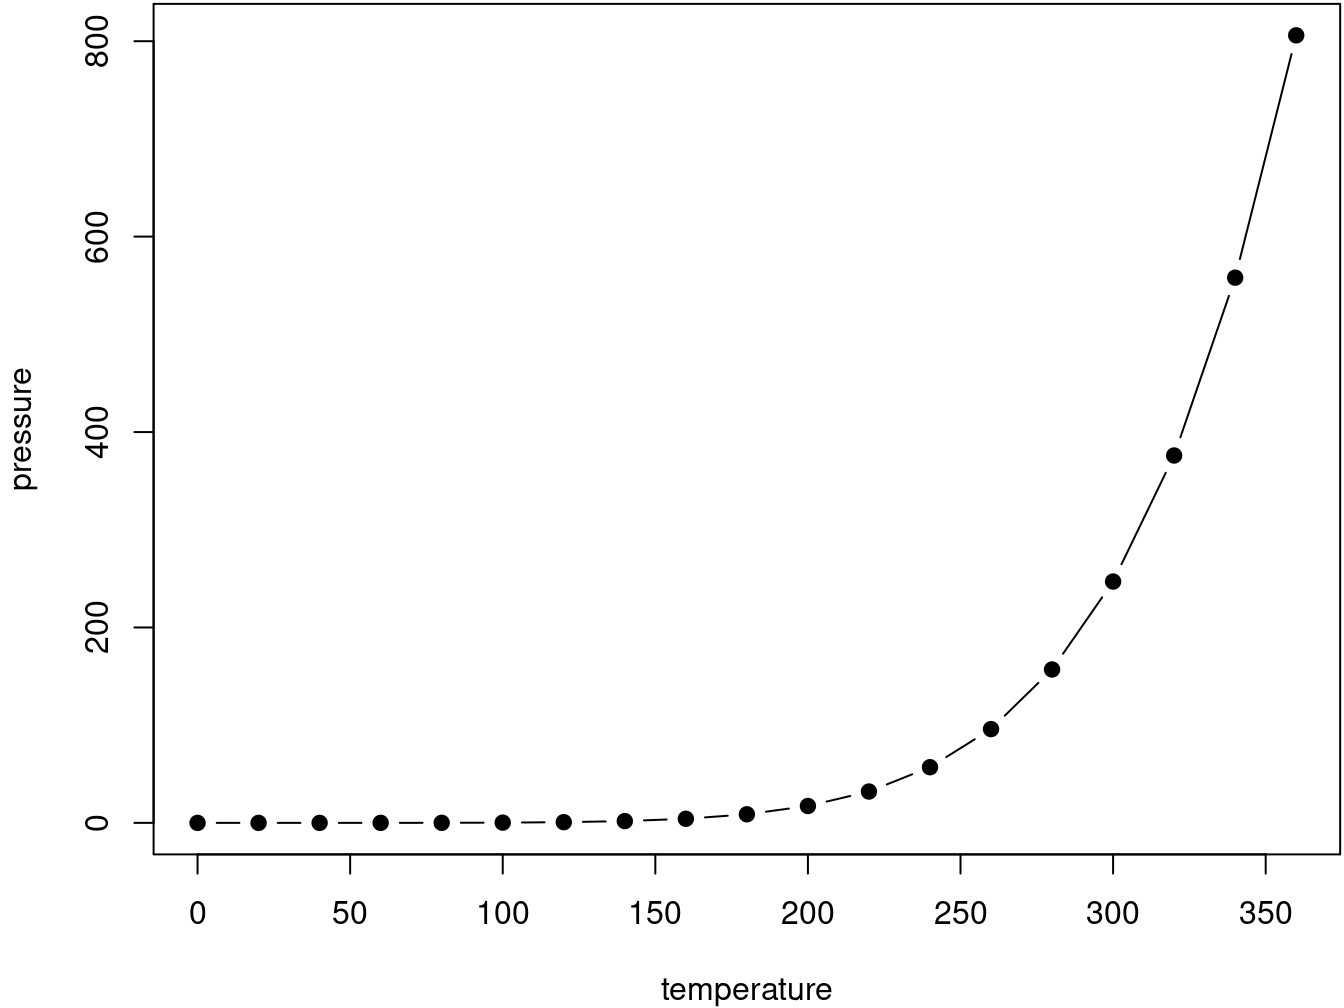
\includegraphics[width=0.8\linewidth]{data-science-practices-1_files/figure-latex/nice-fig-1} 

}

\caption{Here is a nice figure!}\label{fig:nice-fig}
\end{figure}

Reference a figure by its code chunk label with the \texttt{fig:}
prefix, e.g., see Figure \ref{fig:nice-fig}. Similarly, you can
reference tables generated from \texttt{knitr::kable()}, e.g., see Table
\ref{tab:nice-tab}.

\begin{Shaded}
\begin{Highlighting}[]
\NormalTok{knitr}\OperatorTok{::}\KeywordTok{kable}\NormalTok{(}
  \KeywordTok{head}\NormalTok{(iris, }\DecValTok{20}\NormalTok{), }\DataTypeTok{caption =} \StringTok{'Here is a nice table!'}\NormalTok{,}
  \DataTypeTok{booktabs =} \OtherTok{TRUE}
\NormalTok{)}
\end{Highlighting}
\end{Shaded}

\begin{table}

\caption{\label{tab:nice-tab}Here is a nice table!}
\centering
\begin{tabular}[t]{rrrrl}
\toprule
Sepal.Length & Sepal.Width & Petal.Length & Petal.Width & Species\\
\midrule
5.1 & 3.5 & 1.4 & 0.2 & setosa\\
4.9 & 3.0 & 1.4 & 0.2 & setosa\\
4.7 & 3.2 & 1.3 & 0.2 & setosa\\
4.6 & 3.1 & 1.5 & 0.2 & setosa\\
5.0 & 3.6 & 1.4 & 0.2 & setosa\\
\addlinespace
5.4 & 3.9 & 1.7 & 0.4 & setosa\\
4.6 & 3.4 & 1.4 & 0.3 & setosa\\
5.0 & 3.4 & 1.5 & 0.2 & setosa\\
4.4 & 2.9 & 1.4 & 0.2 & setosa\\
4.9 & 3.1 & 1.5 & 0.1 & setosa\\
\addlinespace
5.4 & 3.7 & 1.5 & 0.2 & setosa\\
4.8 & 3.4 & 1.6 & 0.2 & setosa\\
4.8 & 3.0 & 1.4 & 0.1 & setosa\\
4.3 & 3.0 & 1.1 & 0.1 & setosa\\
5.8 & 4.0 & 1.2 & 0.2 & setosa\\
\addlinespace
5.7 & 4.4 & 1.5 & 0.4 & setosa\\
5.4 & 3.9 & 1.3 & 0.4 & setosa\\
5.1 & 3.5 & 1.4 & 0.3 & setosa\\
5.7 & 3.8 & 1.7 & 0.3 & setosa\\
5.1 & 3.8 & 1.5 & 0.3 & setosa\\
\bottomrule
\end{tabular}
\end{table}

You can write citations, too. For example, we are using the
\textbf{bookdown} package \citep{R-bookdown} in this sample book, which
was built on top of R Markdown and \textbf{knitr} \citep{xie2015}.

\hypertarget{scratch-pad}{%
\chapter{Scratch Pad of Loose Ideas}\label{scratch-pad}}

\hypertarget{chapters-sections-to-form}{%
\section{Chapters \& Sections to Form}\label{chapters-sections-to-form}}

\begin{enumerate}
\def\labelenumi{\arabic{enumi}.}
\tightlist
\item
  Tools to Consider

  \begin{enumerate}
  \def\labelenumii{\arabic{enumii}.}
  \tightlist
  \item
    tidyverse
  \item
    odbc
  \end{enumerate}
\end{enumerate}

\bibliography{book.bib,packages.bib}


\end{document}
